%\documentclass[a4paper, 10pt]{article}
\documentclass[10pt]{article}
\usepackage[brazil]{babel}
\usepackage[utf8]{inputenc}
\usepackage{listings}
\usepackage{color}
\usepackage{amsthm}
\usepackage{graphicx}
\usepackage{schemabloc}
\usepackage{cite}
\usepackage{hyperref}
\usetikzlibrary{circuits}
\setlength{\parindent}{0pt}
\setlength{\parskip}{18pt}
\usepackage{cleveref}
\usepackage{steinmetz}

\title{Motor de Indução Gaiola de Esquilo}
\author{Felipe Bandeira da Silva\\1020942-X}
%\date{}

\begin{document}


\maketitle

%\newpage

%\begin{abstract}
\textit{Este laboratório tem como objetivo: Analisar as estruturas de indução trifásico de gaiola de esquilo. Determinar suas características de partidad a vazio e com máxima carga.}
%\end{abstract}

\newpage

\tableofcontents

\newpage

%\listoffigures


%%%%%%%%%%%%%%%%%%%%%%%%%%%%%%%%%%%%%%%%%%%%%%%%%%%%%%%%%%%%%%%%%%%%%%%%%%%%%%%%
% fundamentação teórica
\newpage
\section{Introdução}

Os motores do tipo gaiola de esquilo são, os mais utilizados
no campo industrial, os mais fáceis na manutenção. Também
conhecidos como motores de indução ou simplesmente como \textbf{MIT}.
O nome gaiola de esquilo vem da construção interna do 
rotor, que apresenta uma formação geométrica muito similar
a uma gaiola de esquilo, gaiola esta bastante conhecida 
na cultura norte americana. 
O estator é composto basicamente de laminas de aço magnético, com tratamento químico para a redução da perdas por correntes parasitas e histerese. São chapas com formador de anéis com ranhuras internas, ranhuras onde são alojadas os enrolamentos. Este que é curto circuito para promover o movimento contra magnético produzido pelo estator. O motor de indução tem o seu principio nos meados do seculo 19.
Quando um francês François Arago formulou que existe uma campo magnético rotativo nos campos. Tais campos produzidos por maquinas usadas no processamento de alimentos, onde as forças eram promovidas por corrente de aguas. Algo que não era prático. Já em 1885, o engenheiro Nikola Tesla, desenvolveu e trabalhou em um motor de indução, neste relatório conhecido como motor de indução gaiola de esquilo, que foi demostrado o seu pleno funcionamento em 1887. Onde Tesla ganhou patente em cima de sua ideia.

Tesla então introduz na industria uma nova tecnologia, simples, barata e bastante robusta quando se trata de movimentos rotacionais. Descrevendo em seu paper um motor de quatro polos trifásico, com um rotor alimentado com corrente continua. George Westinghouse então desenvolve uma solução mais simples, que necessita apenas de corrente alternada, licenciada com base nas ideias de Nikola Tesla. Em 1986, duas grandes empresas norte americanas, General Eletric e Westinghouse firma um contrato para que o motor de indução seja chamado de motor de indução Gaiola de Esquilo.

O principio de operação esta ligado com a força contra magnética promovida pelo rotor, que este uma fez dentro de um campo magnético esta submetido a uma indução. O Fechamento das bobinas do rotor provoca essa foram contrária. O fator de escorregamento está presente e, é responsável pelo inicio da rotação do motor. 

A velocidade síncrona do motor é definido pela equação \ref{eq:velocidademotorsincorno} e é dada em RPM.

\begin{equation} \label{eq:velocidademotorsincorno}
n_s = \frac{120 f}{p}
\end{equation}

A fator de escorregamento é definido pela equação \ref{eq:fatordeescorregamento}.

\begin{equation} \label{eq:fatordeescorregamento}

s = \frac{n_s - n_r}{n_s}

\end{equation}

Onde $n_r$ é conhecida como 
a velocidade mecânica do rotor. 

As vantagens da gaiola de alumínio segundo a GE esta em, as tensões das barras mantém a compress]ap do pacote de lâminas. Como a gaiola pode ser 
produzida pelo processo de fundição as dimensões das barras são livre e 
dependentes apenas dos cálculos do projetista e limitações na produção.
A resistência elétrica do rotor é maior entretanto o custo de produção
é menor do que os rotores que usam cobre.

Um gaiola de cobre é responsável pela redução das perdas no rotor $14 \%$
a $20 \%$. A temperatura de trabalho é reduzida.

A figura abaixo exemplifica um motor de indução

\begin{figure}[!ht]
    \centering
    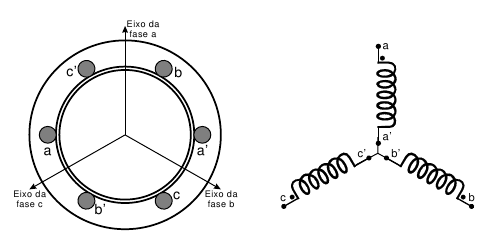
\includegraphics[scale=0.8]{seccaotransversalmaquinas}
    \caption{Secção transversal de uma maquina assíncrona.}
    \label{fig:motorutilizado}
\end{figure}

\section{Variando a carga aplicada}

A primeira parte da prática do laboratório consiste em ligar uma carga, eletrodinamômetro. 
Mensurar as corrente e tensões para obter potência elétrica do motor. O circuito montado esta na figura 4.1 do caderno de praticas. 

Uma fez feita a experiência, a tabela abaixo mostra os valores numéricos obtidos com a prática.

\begin{center}
    \begin{tabular}{c|c|c|c|c|c|c}
            Conjudado(lbf.in) & $I_1$ & $I_2$ & $I_3$ & $WATTs$ & $VARs$ & Velociade \\
            \hline
            0 & 0.658 & 0.742 & 0.647 & 100 & 210 & 1780 \\
            3 & 0.715 & 0.850 & 0.699 & 160 & 220 & 1760 \\
            6 & 0.844 & 1.002 & 0.820 & 240 & 230 & 1740 \\
            9 & 1.003 & 1.196 & 0.995 & 300 & 250 & 1700 \\
            9 & 1.229 & 1.440 & 1.221 & 300 & 260 & 1650 \\
    \end{tabular}
    \captionof{table}{}
\end{center}

Os valores para as potências ativas em 9 e 12 libras força, ultrapassaram
os 300 watts possíveis que o equipamento media.

\section{Corrente de partida}

O teste agora é feito para a situação onde o motor está 
sujeito a uma carga extremamente alta, no inicio de funcionamento.
Estes valores são medidos de forma apenas aparente e rapidamente. 
Para que o motor não sofra nenhuma avaria em sua estrutura.

Os valores foram mensurados e são apresentados na tabela abaixo, 

\begin{center}
    \begin{tabular}{c|c}
        Grandeza & Valores \\
        \hline
        $I_1$ & 4.3 A \\
        $E_1$ & 210 V \\
        Torque & 0.19 lbf.in \\
    \end{tabular}
    \captionof{table}{}
\end{center}

A potência aparente para este conjugado de partida é de 1.564 KVA.

\section{Conclusão}

Concluímos com este trabalho a verdadeira importância de um 
motor de indução do tipo Gaiola de Esquilo. Percebe-se que o
motor com a mesma potência elétrica, consegue desenvolver 
mais potência mecânica. Que outros motores. É bastante estável.
Com isto um motor com alto grau de robustez. Percebe-se então
porque o motor de indução tipo gaiola de esquilo foi responsável
pela segunda revolução industrial.
A ultima experiência, que tratou da corrente de partida do motor
mostrou que o mesmo apresenta uma alta corrente de partida em 
relação ao de roto bobinado. Mostrou também a dificuldade de 
controle de velocidade que o mesmo apresenta. Um baixo fator
de potência indutivo. 
\end{document}

